%! Author = Vojta
%! Date = 21.10.2021

\chapter{Technologie}

\section{Výběr}
Vzhledem k tomu, že aplikace byla původně zamýšlena jako osobní projekt, který by si následně spravoval sám vedoucí a já
jsem měl zkušenosti pouze s frameworkem Vue.js, hlavní technologie, okolo které se projekt postaví, byla předem daná. Poté
jsem postupně vybíral další součásti, které bychom mohli využít. Velkou výhodou bylo, že právě vedoucí práce má s většinou
z těchto knihoven či pluginů zkušenosti, a tak když se mi něco nedařilo, mohl jsem se na něj obrátit.

\section{Vue.js}
Vue je progresivní JavaScriptový framework, který narozdíl od konkurenčních řešení (React, Angular) nezaštiťuje žádná velká
korporace, ale je vyvíjen komunitou.\cite{VueJS} Zvolil jsem verzi 3, protože je to lepší řešení do budoucna, než později aktualizovat
celou aplikaci z verze 2. V pozdější fázi vývoje se ale ukázalo, že pro verzi 3 nebyla plně dokončena hlavní knihovna, kterou jsem chtěl využít.
Musel jsem tak ponížit verze všech závislostí a přejít tak na verzi 2.

\section{Vuetify}
Vuetify je knihovna implementující různé komponenty, které je možné použít při tvorbě uživatelského rozhraní. Kromě toho
usnadňuje práci s rozložením na stránce, přizpůsobením barevného téma, ikonami atd. Další výhodou jsou týdenní aktualizace
momentální verze, které přidávají nové funkce a opravují nalezené chyby.\cite{VuetifyWhy}
Bohužel tato knihovna nebyla v době vývoje plně dokončena a byla pouze v alpha verzi, tudíž spoustu věci nefungovalo jak by mělo.
% TODO

\section{Vuex}
Knihovna Vuex~\cite{Vuex} se využívá pro uložení stavu aplikace. Je vhodné ji využít u dat, která jsou využívána na více místech a jejich
předávání skrz komponenty by bylo jinak složité.

Změna či přístup k stavu a všechny operace nad ním se řeší ve speciálním souboru, kde se Vuex inicializuje. K těmto operacím využijeme \emph{state, mutations, getters, actions a modules}.
\emph{State} označuje strukturu dat, tedy pokud potřebuji nějak zaznamenávat recepty, vytvořím zde pole či objekt a s ním dále pracuji. Pro to abych přidal recept využiji \emph{actions} v kombinaci s
\emph{mutations}. \emph{Actions} je obal funkcí, které můžu zavolat odkudkoliv z aplikace a ty provedou nějakou změnu nad daty. Například data stáhnou, aktualizují nebo nastaví hodnotu, kterou uživatel
zadá. Mutations poté vyvoláme pomocí funkce \mintinline{js}|commit|. Té předáme název mutace, která se má zavolat a tzv. \emph{payload}, tedy data, která chceme do stavu zapsat. Mutace již poté pouze zapíše
do stavu a nic dalšího by řešit neměla.

Pro získání stavu lze využít \emph{getters}. V těchto funkcích by také neměla být žádná další logika, ačkoliv se zde dá vytvořit drobné filtrování či řazení.
Když se aplikace rozroste a obsahuje mnoho dat, tak aby všechny tyto části byly přehledné, je možné vytvořit více modulů a spravovat data která mají něco společného
odděleně. Samotné moduly se pak naimportují do \emph{modules} a jsou přístupné v celé aplikaci.

\section{Vue i18n}
I18n~\cite{i18n} je rozšíření pro překlady, díky kterému je možné texty v aplikaci napsat v několika jazycích. Nejprve jsem tvořil aplikaci dvojjazyčně
v angličtině a čestině, ale nakonec jsem se rozhodl, že prozatím dává aplikace smysl pouze v češtině. Nicméně překlady jsem ponechal a v budoucnu
je možné je využít.

\section{Firebase}
Firebase~\cite{Firebase} je platforma pro vývoj aplikací. Nabízí spoustu produktů, které je možné využít a tím zjednodušit vývoj.
Dané produkty mohou mezi sebou komunikovat a reagovat na různé události. Firebase poskytuje multiplatformní SDK, což znamená, že je
možné vyvíjet v několika programovacích jazycích jako je Java, Kotlin, Swift, JavaScript nebo C++. V kombinaci s touto platformou je možné
využít další nástroje od společnosti Google, jako jsou Analytics, Google Ads a další. K tomu lze přidat rozšíření, které vyžadují jen základní
konfiguraci a propojí aplikaci s dalšími externími systémy, jako je Stripe~\cite{Stripe} či Algolia~\cite{Algolia}.

\subsection{Ceny}
Firebase má velikou výhodu v tom, že je zdarma, pokud uživatelé nevyčerpají určitý objem dat či přístupů k databázi. Tato kapacita se resetuje
denně nebo měsíčně, podle toho o jaký podsystém se jedná. V nabídce jsou dva plány. První \emph{Spark Plan} je úplně zadarmo, ale má určitá omezení.
Na druhou stranu \emph{Blaze Plan} má stejné limity a platí se pouze za jejich překročení. Tedy například pro databázi Firestore je zdarma padesát tisíc
čtení denně pro oba plány a pro \emph{Blaze Plan} poté stojí každých dalších sto tisíc čtení 1,40 Kč.~\cite{FirebasePricing}

\subsection{Firestore}
Cloud Firestore~\cite{Firestore} je NoSQL dokumentová databáze. Narozdíl od SQL databází, které se soustředí na snížení duplikace dat, se dokumentová
databáze zaměruje na časté aktualizace a změny. Největší rozdíl mezi těmito typy je způsob uložení dat. SQL reprezentuje data pomocí
tabulek s řádky a sloupci, dokumentová databáze má JSON dokumenty a jejich kolekce. To vede k flexibilnějšímu datovému modelu, rychlejším
dotazům a lehčímu vývoji pro vývojáře.~\cite{MongoDBNoSQL}

Firestore nabízí vlastní řešení bezpečnosti přes Firebase Rules, které více přiblížím v kapitole o implementaci pomocí ukázek.

\subsection{Storage}
Cloud Storage je uložiště, kam je možné ukládat různé soubory, které uživatelé poutřebují při používání aplikace. V mém případě to
budou fotografie jídel či surovin. Pro ukládání dat se používají takzvané \emph{Cloud Storage buckets}, což jsou pouze kontejnery,
které můžeme využít tak, aby data byla organizovaná~\cite{FirebaseBucket}. K tomu lze vytvořit vnitřní strukturu pomocí složek nebo
data oddělit podle jejich provázanosti do různých kontejnerů.

\subsection{Hosting}
Webová aplikace musí být někde dostupná, aby k ní uživatelé mohli přistoupit. K tomu lze v rámci Firebase využít \emph{Hosting}.
Ten nabízí rychlé SSD disky, na kterých web běží, SSL certifikáty pro vlastní domény zdarma, jednoduchý \emph{deploy} nebo náhledy
aplikace předtím než je nasazena na produkci.~\cite{FirebaseHosting}

\subsection{Functions}
Firebase Cloud Functions mají za úkol vývojářům ulehčit vývoj backendu tak, aby nemuseli řešit záležitosti okolo správy serverů.
Funkce, které na tomto systému běží mohou reagovat na širokou škálu událostí uvnitř Firebase produktů. Například pokud se do aplikace
přihlásí nový uživatel, může se spustit funkce, která mu odešle uvítací email. Jako programovací jazyk se pro psaní funkcí použivá Node.js.~\cite{FirebaseFunctions}

\section{Fulltextové vyhledávání}
Při práci s Firebase jsem zjistil, že při dotazování se na záznamy není možné filtrovat podle názvu
(abych byl přesný, možné to je, ale není to vhodné). Po zkoumání dokumentace, jsem našel stránku s doporučením pro
fulltextové hledání. V nabídce byla tři řešení.~\cite{FulltextSearch}

\begin{itemize}
    \item Elastic
    \item Algolia
    \item Typesense
\end{itemize}

Problém jsem řešil s vedoucím a přišli jsme na několik možných řešení sami. Stáhnout si data o všech receptech ve formátu
\emph{id:name} a poté filtrovat výsledky hledání na FE. Dále bychom mohli použít Firebase Cloud Functions, kde bychom
využili hashování. Nakonec jsem se ale rozhodl, že využiji jedno z nabízených řešení přímo Googlem.

Vybral jsem Algolii~\cite{Algolia}, kvůli dobré podpoře Vue a Firebase, nejmenší složitosti implementace a bezplatnému základnímu plánu.

Při vývoji jsem ale zjistil, že základní režim (tedy 10 000 čtení za měsíc) nejspíše stačit nebude. Nakonec jsem proto přešel na
frontendové vyhledávání. Všechna data jsem stáhnul při načtení aplikace a poté s nimi dál pracoval.

\section{Vue Router} % TODO: Více rozepsat
V aplikaci je potřeba mít navigaci. Ve Vue se používá Vue Router~\cite{VueRouter}, který umožní pohyb po různých stránkách.

\subsection{SPA}
SPA neboli \emph{single page application} je stránka, která využívá takové architektury, kde použitá technologie nejen kontroluje
vzhled stránky, ale i data a manipulaci s nimi a navigaci tím způsobem, že není nutné provádět obnovení stránky.\cite{VueSPA}

Pro demonstraci rozdílu mezi MPA a SPA jsem zvolil následující diagramy.

\begin{figure}[H]
    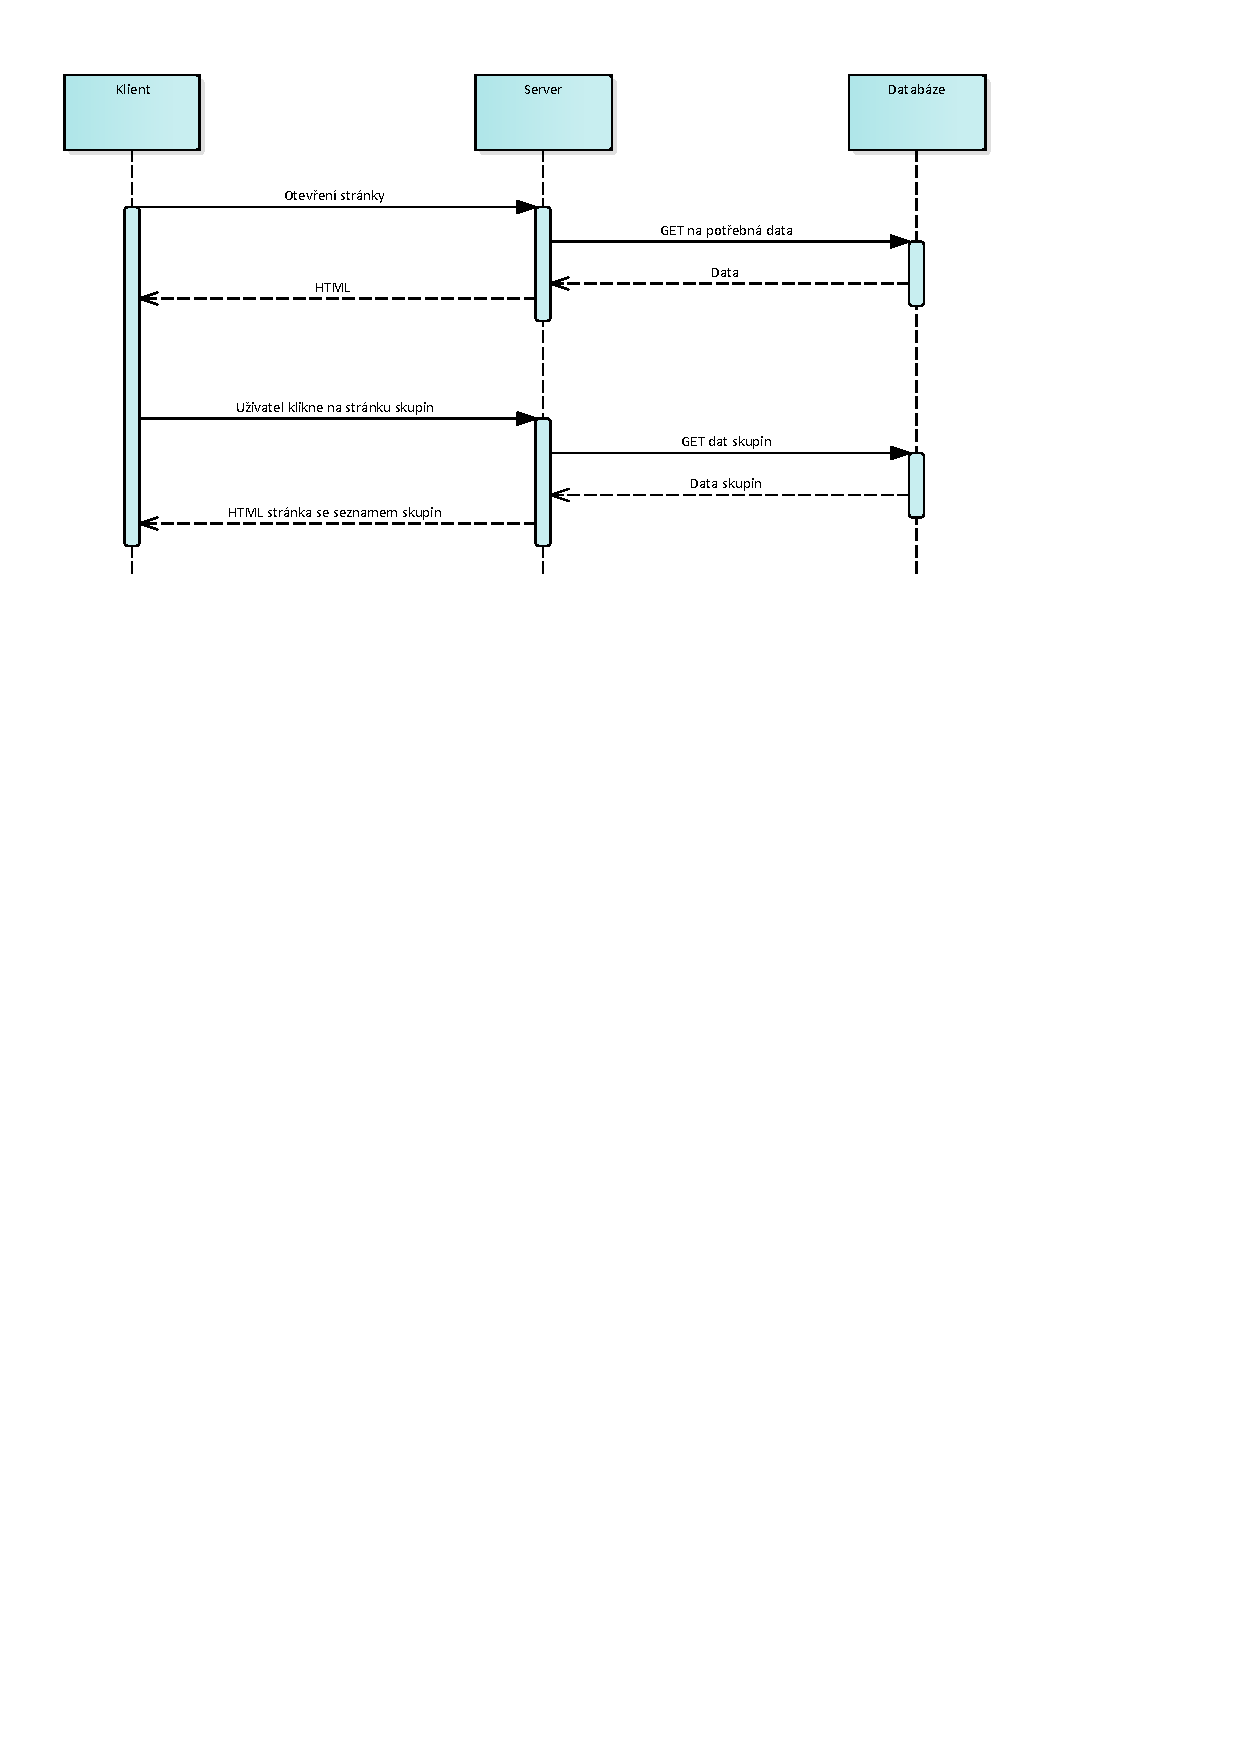
\includegraphics[width=\textwidth]{pdf/MPA-model}
    \caption{MPA Model} \label{picture:recipeo:mpa-model}
\end{figure}
\begin{figure}[H]
    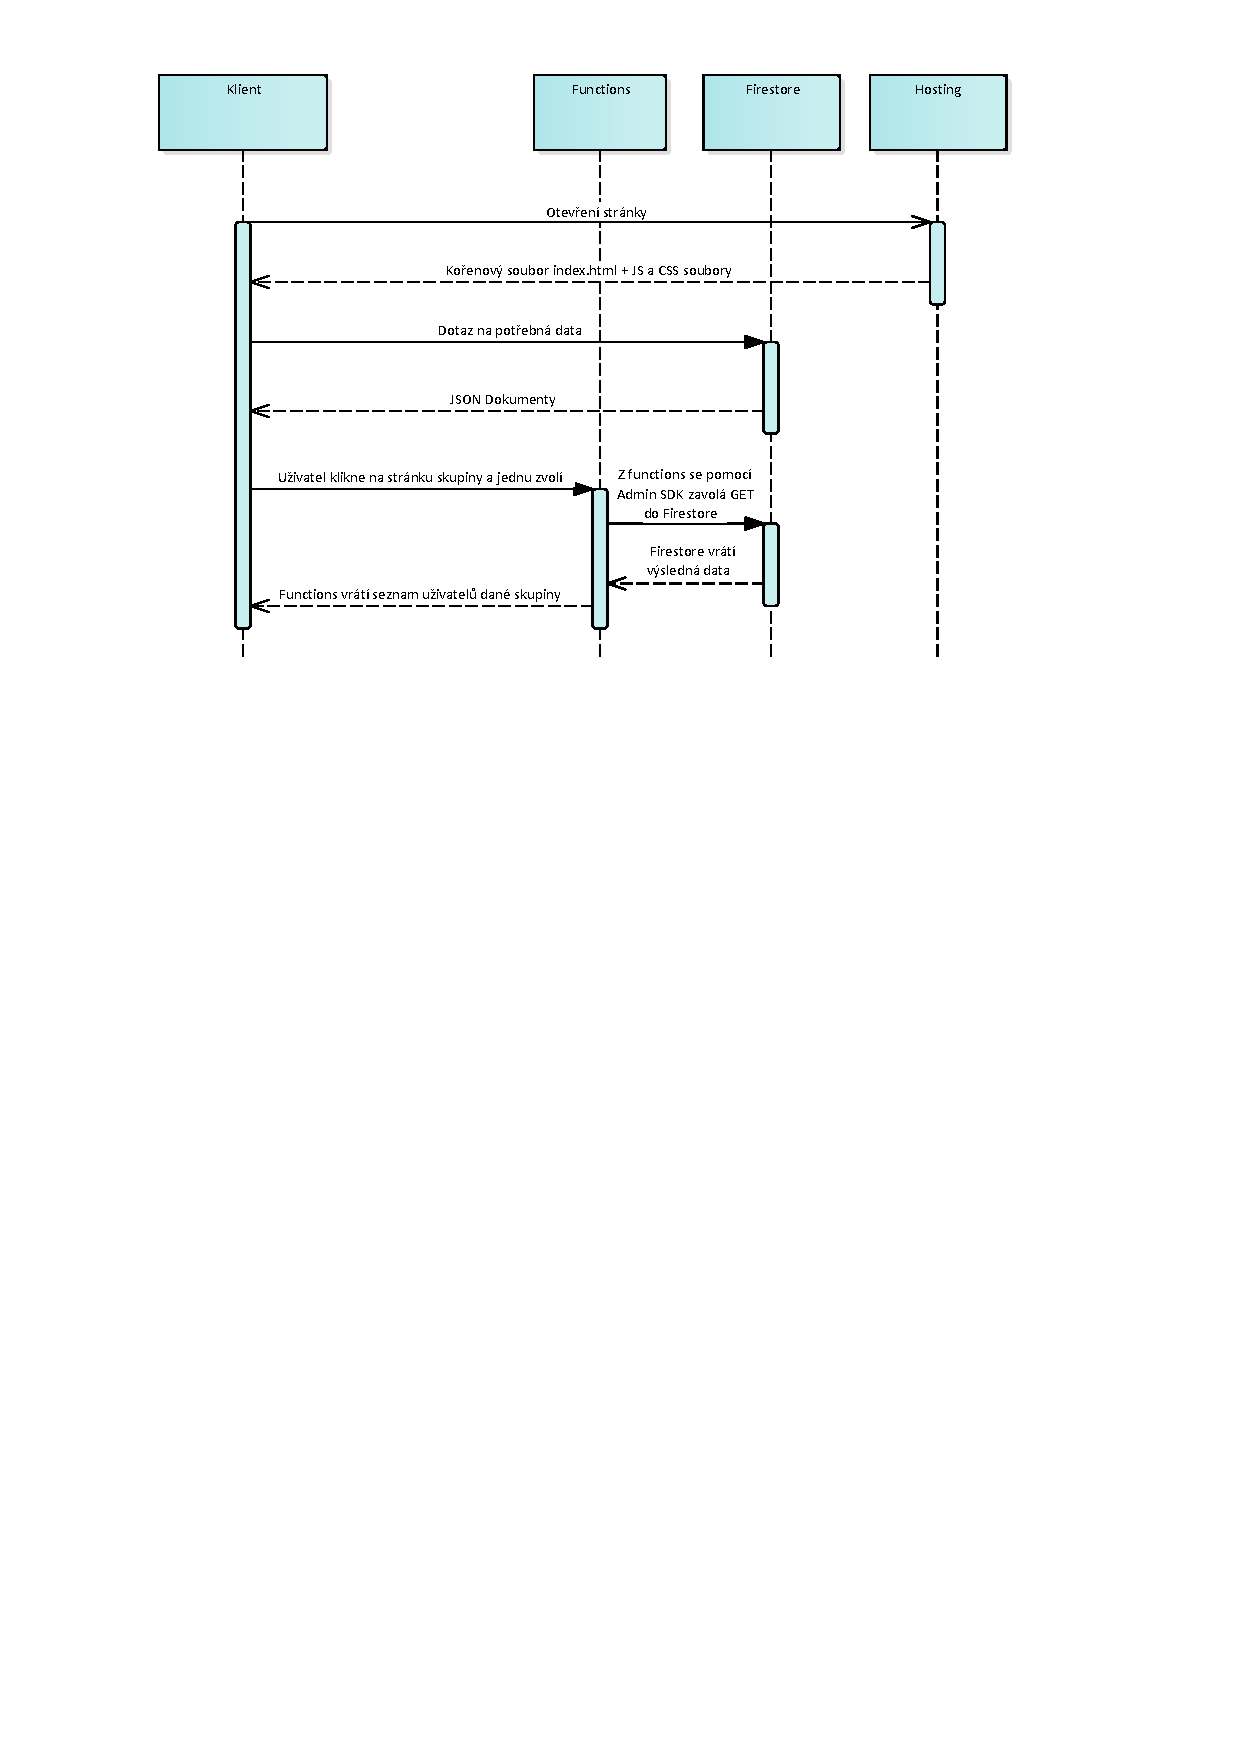
\includegraphics[width=\textwidth]{pdf/SPA-model}
    \caption{SPA Model} \label{picture:recipeo:spa-model}
\end{figure}

Jak je ve SPA diagramu vidět, některá data lze získat přímým přístupem do Firestore, ale jiná je nutné stáhnout z Functions.
Je to dané tím, že u některých dat není možné ošetřit jejich bezpečnost pomocí Firestore Rules a je tedy nutné k nim přistupovat
přes Functions, které má dostupné Admin SDK, tedy neomezený přístup k celé databázi. Data tak mohou být pro běžné uživatele nepřístupná,
ale pomocí volání cloudové funkce přímo z aplikace je možné je stáhnout. Také se dají data tímto způsobem předzpracovat, což může
být výhodné právě z hlediska bezpečnosti a k uživateli se tak nedostane nic co by nemělo.

\section{PWA}

Progresivní webová aplikace se snaží usnadnit vývoj standardních webových aplikací jako nativní aplikace pro mobilní telefony.
K tomu využívá \emph{service workers} a webové aplikační \emph{manifesty}. Aby se aplikace dala považovat za PWA, měla by
mít tyto vlastnosti~\cite{PWAAckee}.


\begin{itemize}
    \item Progresivní

    Je použitelná na starších prohlížečích s určitými omezeními, ale plně funkční na nejnovějších verzích prohlížečů.
    \item Responzivní

    Stránka je optimalizována pro všechny typy obrazovek (od nejmenších telefonů, přes notebooky až po velké PC monitory)
    \item Nezávislá na konektivitě

    Pomocí technologie \emph{service workers} je možné aplikaci využívat offline díky cachování
    \item App-like

    Aplikace vypadá jako nativní ačkoliv na pozadí je webová aplikace
    \item Aktuální

    Poskytují vždy aktuální verzi díky procesu update technologie \emph{service workers}
    \item Zabezpečená

    Výhradní použití HTTPS zamezí odposlouchávání či jiné manipulaci s přijímanými daty
    \item Znovuzapojení uživatele

    Je možné využít funkce push notifikace, která poté uživatele naláká zpět do aplikace \footnote{Tyto push notifikace z webového prohlížeče jsou již několik let běžnou
    záležitostí na systému Android, ale do iOS od společnosti Apple se dostaly teprve nedávno~\cite{PWANotifications}.}
    \item Instalovatelná

    Při přístupu na stránku je uživateli nabídnuto si aplikaci stáhnout, poté k ní může přistupovat jako k nativní aplikaci
    \item Odkazovatelná

    Dá se na ní jednoduše přistoupit pomocí URL bez nustnosti instalace
\end{itemize}
